\section{Applications}
\label{sec:app}

In order to test the abilities proposed for memcomputers, \citep{DiVentra:2012fh} did an experiment with the problem of finding the shortest path.
The problem of the shortest path is the procedure of finding a way to connect two points in a matrix via the shortest path of points between them.
It is known that this problem has complexity of logarithmic time \cite{shortestPath}.

The proposed memcomputer architecture is a square matrix made of memelements with resistive characteristic, as shown in Figure \ref{fig:square}.
Here, the architecture is a non-programable computer with memelements connected in a square format to each other.
It is worth mentioning that this memcomputer is specifically projected to solve the shortest path, that is it is not programmable for other functionalities other than that.
Also, notice that each memelement has a switch attached to it, which provides the possibility of writing and reading individually.
This is requires for initialization purposes as well as reading the result after the computation.

\begin{figure}[hbt]
    \begin{center}
    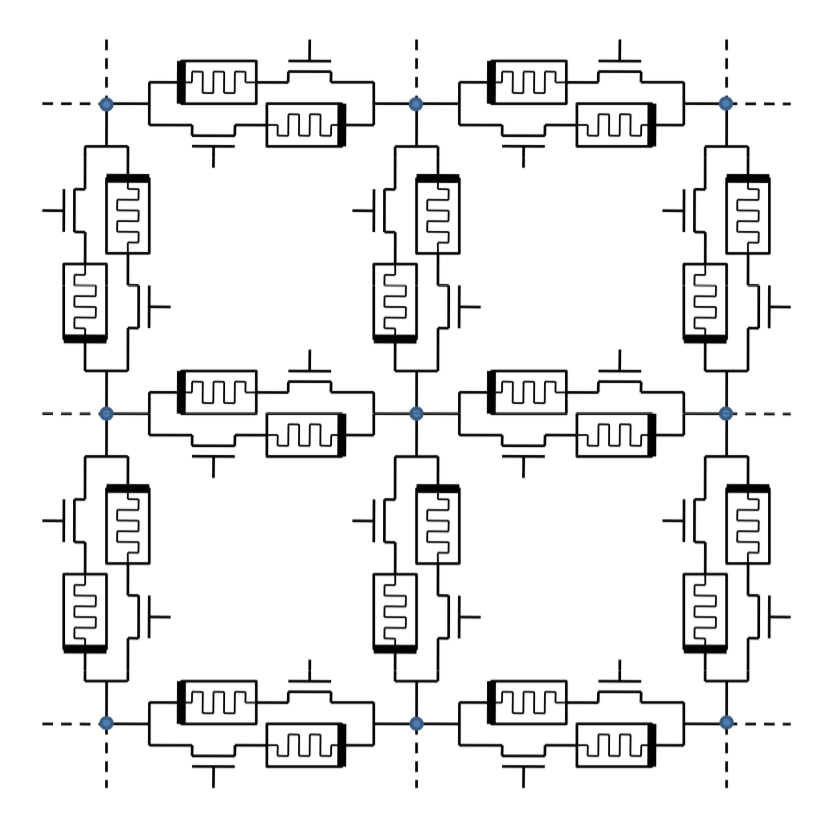
\includegraphics[width=0.5\textwidth]{figures/memcomputer.png}
    \caption{A memcomputer proposed in \citep{DiVentra:2012fh} for solving the shortest path problem.}
    \label{fig:square}
    \end{center}
\end{figure}

In this computer, we give the inputs by activating a subset of points in this grid, that is by applying a voltage in a subset of memelements.
The processing part is the collective evolution of the states of the memelements after the input is applied.
Lastly, the result of the processing step is the final state of all memelements.

The shortest path problem can be be computed using the memcomputer in Figure \ref{fig:square} by applying a constant voltage to two points the square.
These are the required input.
The memelements closer to the application of the voltage is affected by the electron current around.
Therefore, the memelement changes its resistance by lowering it down, that is the memelement become active.
The closest memelement activates itself similarly, forming a reinforcement path.
In this way, a path from the first application point to the second one is formed.
The final state that can be read from the memcomputer is a straight line of active memelements from the first point to the second one, which is the shortest path in this square.